\section{序論}
\subsection{はじめに}
低温で物質が超伝導を示すことは1911年にオランダのH. K. Onnesにより水銀で発見された。のちにこの現象は多くの物質に普遍的であることが分かり、すでに数千種類の超伝導体が発見されている。超伝導状態にある物質は電磁気学的および熱力学的に特徴的な振る舞いを見せる。もっとも典型的な性質は電気抵抗がゼロとなることであり、散逸のない電流ケーブルや強力な電磁石に応用されている。また磁場に対する応答も、完全に磁場を遮蔽するMeisner効果が一部の金属で現れるなど、金属状態の磁性と劇的に異なる。さらに超伝導体同士を弱く結合すると、巨視的な位相に依存して、Josephson電流と呼ばれる超伝導状態に特有な電流も観測できる。この効果は高感度な磁気センサなどに用いられる。さらに超伝導状態の金属と通常の金属の間の転移の際に比熱に飛びが現れるなど、熱的な振る舞いにも特徴がある。これらの特徴的な物理特性と応用の多彩さから、100年以上に渡り超伝導物理学は物理学の中心的なテーマであり続けてきた。

超伝導物理学の歴史で特に重要なのは、J. G. BednorzとK. A. M\"ullerによる銅酸化物超伝導体の発見である\cite{Bednorz}。銅酸化物超伝導体は母物質の元素置換により超伝導を発現する\cite{Lee2006}。発見以来、多くの人々が元素置換による超伝導物質の探索を行い、液体窒素温度で実現する高温超伝導体\cite{Wu}や、超伝導転移温度$\rm T_c=26K$の鉄系超伝導体\cite{Kamihara}などの異なった物質群も次々に発見された。これらは、いわば化学的な超伝導へのアプローチの成果であって、一部が応用に進展し、さらに銅酸化物超伝導体を関連する強相関電子系物質と金属-絶縁体転移などの研究も刺激した\cite{Lee2006,Imada}。

一方で単純な化学的アプローチは、狙いの組成で母物質に元素を固溶させるのが難しかったり、外部からの刺激で超伝導性を制御できない。そのため異なった手法も近年盛んに研究され、例えば電界(イオンゲート)効果\cite{Ueno,Ueno2,Ye2009}や薄膜効果\cite{Chiang1900}、非平衡過程\cite{Fausti,Hunt2015,Mitrano2016}、パルス加熱・急冷\cite{oike}を用いた手法などが実現されている。これらの効果を用いると、超伝導体以外の物質と超伝導体をスイッチしたり、超伝導転移温度$T_c$を制御することができる。

筆者らの研究グループは特にパルス加熱・急冷を用いた制御に着目した。後述するようにパルス加熱・急冷を用いた制御は可逆的であり、また光を用いた制御が可能なのでリソグラフィ技術を用いてパターニングできることが期待される。さらにこの手法には新超伝導物質発見の可能性がある。しかし非平衡による超伝導を研究された物質の例は少なく、超伝導発現には高い冷却レートが必要で、いまだ応用と理論的な理解は限定的である。

そこで本研究は新規物質としてスズを用い、パルス加熱・急冷による超伝導体制御を実証することを目指した。スズは286.4Kより高温で正方晶の金属相(βスズ)が安定である。一方286.4Kより低温において立方晶の半導体相(αスズ)が安定だが、βスズを十分に早く冷却すると構造相転移できずβスズも準安定となる。このβスズは臨界温度3.7K以下で超伝導を示す。したがって冷却速度(温度履歴)をコントロールすれば、原理的に超伝導体と半導体間の制御・変換が可能である。

αスズとβスズの特性は大きく異なる。αスズは低温で指数関数的に電気抵抗が大きくなるが、超伝導βスズは抵抗で抵抗がゼロとなる。また光学的な性質も異なる。αスズはエネルギー0.018eV(4.4THz)以下の光を透過するが、βスズは反射する。これらの性質から、半導体中の超伝導回路のパターニングは低損失な電気回路のみならず、プラズモニック回路や量子コンピュータなどに有用であることが期待できる。特にスズは地球上に豊富に存在する元素であり、融点が低く取り扱いやすく、また人体への毒性もない。応用の幅広さと取り扱いの簡単さから、パルス加熱・急冷による半導体スズと超伝導スズの変換は有用であることが期待できる。

\subsection{超伝導体の様々な制御法}
前節で述べたように近年は、様々な超伝導体の制御法が提案されている。本節ではそれらの基礎となっている化学的な元素置換法を説明したあと、本実験と関係の深い光パルスを用いた過渡的な超伝導制御法を述べる。最後に本実験で用いたパルス加熱・急冷を用いた手法に関して述べる。

\subsubsection{元素置換による銅酸化物超伝導体の化学的制御}
本節では銅酸化物超伝導体を例にとって、元素置換による化学的な超伝導制御法を述べる。

銅酸化物超伝導体はMott絶縁体の元素置換により超伝導を発現する\cite{Lee2006}。Mott絶縁体の振る舞いは物質の電子間の相互作用の効果を考慮に入れて説明できる。まずMott絶縁体の基本的な描像に関して述べる。

%バンドの形成
孤立した原子核に束縛された電子は離散的なエネルギー準位をとる。しかし原子同士を近づけてゆくと電子の波動関数が重なり、相互作用の影響でエネルギー準位が分裂する。結晶構造において多数個の原子が周期的に配列するとき、固体中の電子準位は幅のあるバンド(帯)構造をとる。図\ref{fig:band}にの原子間距離とエネルギー準位の関係を模式的に示す。原子間距離が小さくなると電子のエネルギー順位は幅を持つことが読み取れる。
\begin{figure}[!h]
    \begin{center}
   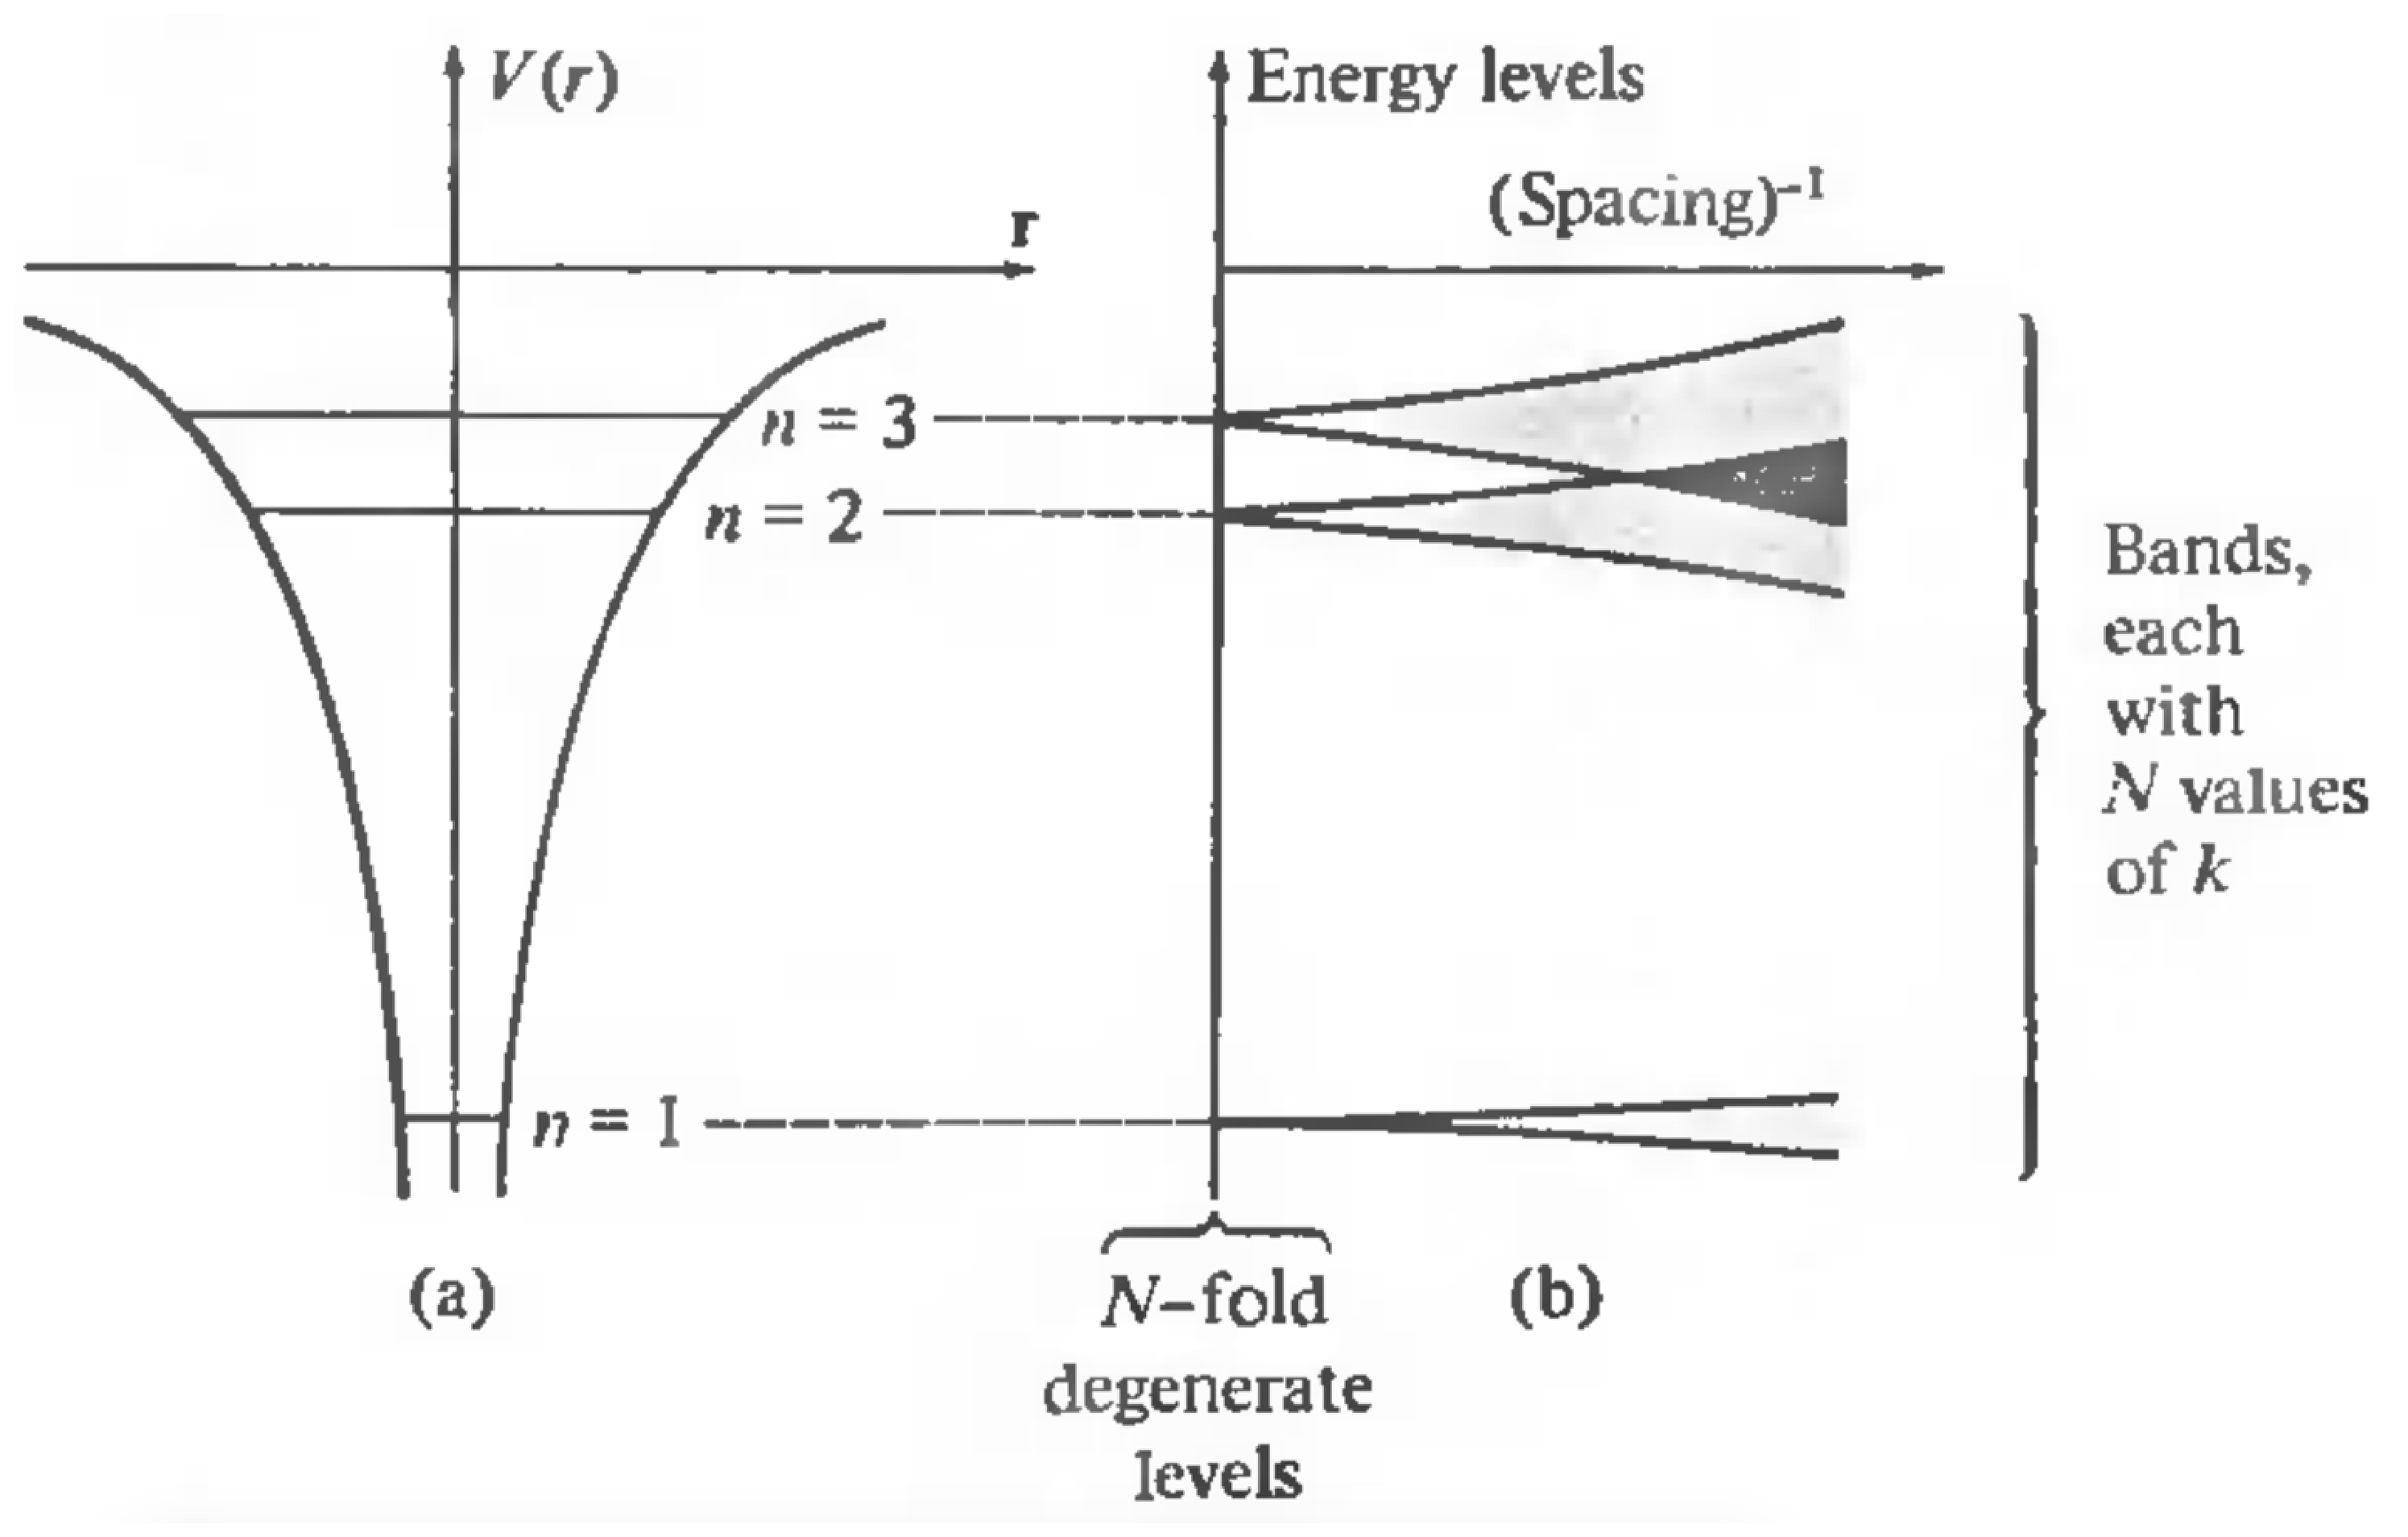
\includegraphics[width=0.7\hsize]{Introduction/band.eps}
  \end{center}
  \caption{原子間距離と電子のエネルギー準位\cite{ashcroft1976}}
  \label{fig:band}
\end{figure}

%ギャップと伝導性
このバンド準位をどのように電子が占有するかだけの情報から固体の多くの性質を説明したのが、(広い意味での)固体のバンド理論である。固体のバンド理論は多くの金属と半導体、絶縁体の性質を説明する。電子がイオンと電荷の中性条件を満たすようにバンド準位を独立に占めていったとき、占有された最大のエネルギー準位の直上に空いた準位があれば、物質は金属となる。一方占有された最大のエネルギー準位の直上に準位が存在しないとき、物質は絶縁体もしくは半導体となる。

%独立電子近似と通常の金属
多くの物質では相互作用の影響をイオンのポテンシャルに取り入れて、あたかも電子が独立に振る舞うかのように扱う近似が妥当である(独立電子近似)\cite{ashcroft1976}。これが(狭い意味での)バンド理論の基礎となる近似である。この近似のもとで単位胞1つあたりの電子数が奇数個だと、必ず最大のエネルギー準位の直上に占有されていない準位が存在するため物質は金属となる。

%Mott絶縁体
しかしMott絶縁体は単位胞1つあたりの電子数が奇数個であるにも関わらず、絶縁体である。この事実はMott絶縁体の電子間のクーロン反発によってギャップ(Mottギャップ)が開くことと言う描像で説明される。すなわち(狭い意味のバンド理論で記述される)通常の絶縁体とMott絶縁体はバンドの形成のされ方が異なる。この描像を模式的に示したのが図\ref{fig:Mott_gap}である。
\begin{figure}[!h]
    \begin{center}
   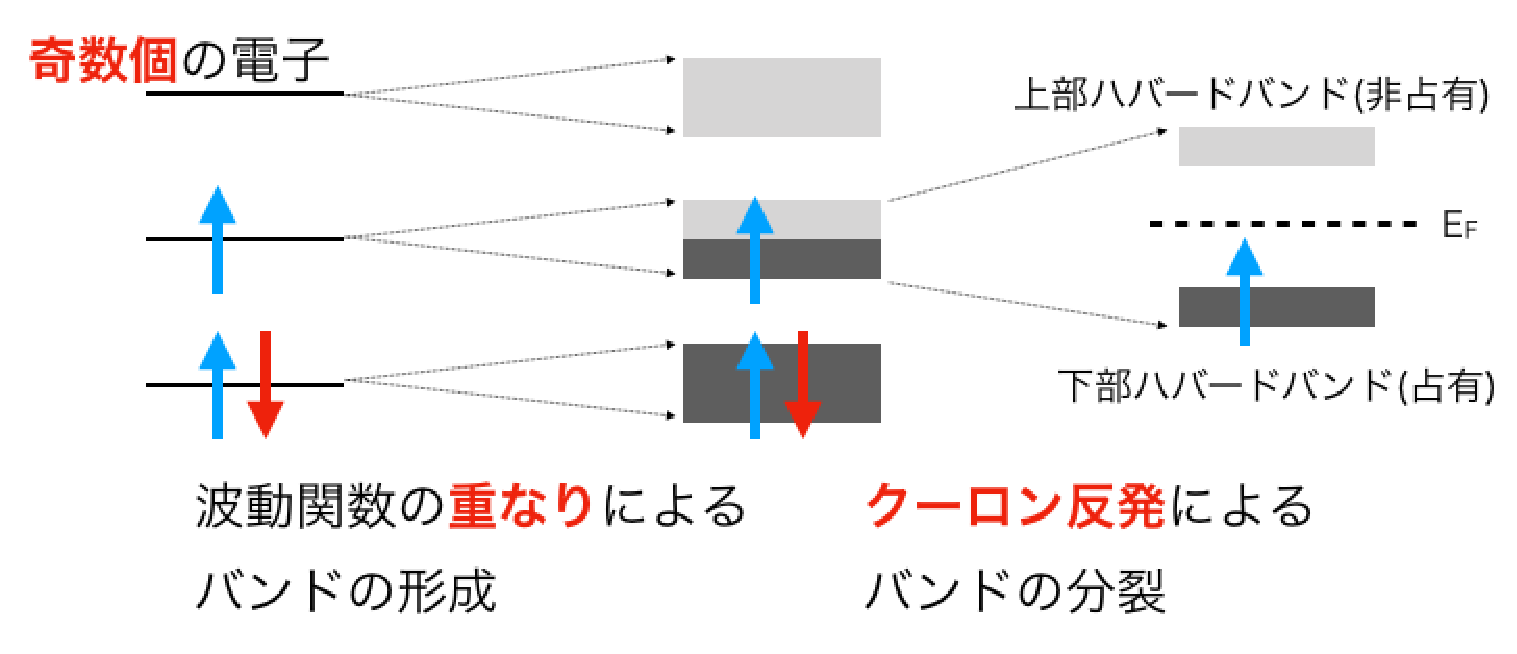
\includegraphics[width=0.6\hsize]{Introduction/Mott_gap.eps}
  \end{center}
  \caption{Mottギャップの形成}
  \label{fig:Mott_gap}
\end{figure}

%Mott絶縁体の元素置換
Mott絶縁体は隣接するスピンがお互いに逆を向く反強磁性体で、スピンが長距離秩序を持った状態(秩序状態)である。このMott絶縁体を元素置換してキャリアをドープすると臨界温度より高温で金属状態が現れる。
図\ref{fig:phase_diagram}に銅酸化物超伝導体の典型的な相図を示す\cite{Andrea2003}。$\rm La_2CuO_4$は反強磁性(AF)のMott絶縁体だが、$\rm Sr$による置換で正孔がドープされ超伝導を示す。ドープ量に対して超伝導転移温度はドーム型の形をしており、あるドープ量で超伝導転移温度は最大となる。$\rm Nd_2CuO_4$も同様に$\rm Ce$による置換で超伝導を示すが、電子がドープされる点が異なる。図に示した二つの相図の特徴は銅酸化物超伝導体に普遍的である\cite{Lee2006}。
\begin{figure}[!h]
    \begin{center}
   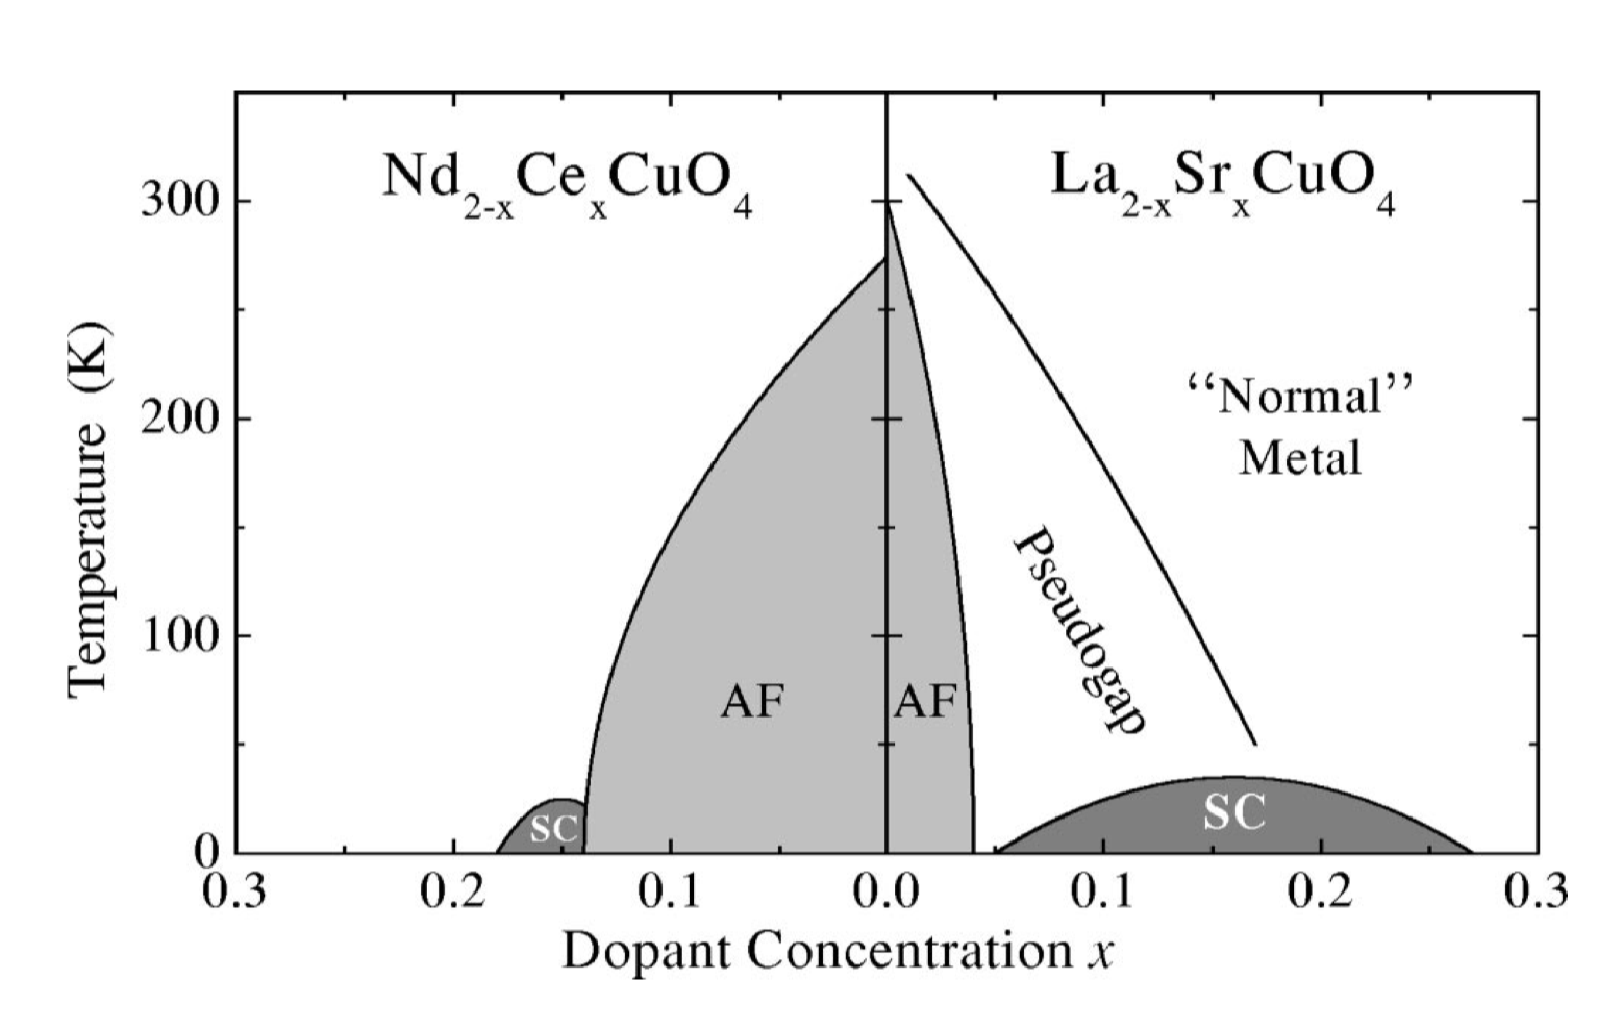
\includegraphics[width=0.6\hsize]{Introduction/phase_diagram.eps}
  \end{center}
  \caption{銅酸化物超伝導体の典型的な相図\cite{Andrea2003}}
  \label{fig:phase_diagram}
\end{figure}

前述したように、母物質のMott絶縁体を元素置換した銅酸化物超伝導は多大な分野に影響を与えた。特に元素置換による化学的な制御法は、電界(イオンゲート)効果による超伝導制御法をもたらした。しかしこれらは平衡過程を用いた手法である。
次に述べる手法は銅酸化物群の一部を動的に制御する可能性を示した。

\subsubsection{赤外光パルスによる超伝導相の過渡的な制御}
Mott絶縁体を元素置換した銅酸化物において、赤外光パルスを印加すると過渡的な超伝導が現れることが近年示された\cite{Fausti,Hunt2015}。

図\ref{fig:phase_diagram2}に彼らが用いた銅酸化物$\rm La_{1.8-x}Eu_{0.2}Sr_{x}CuO_4$の相図を示す\cite{Cavalleri2018}。典型的な銅酸化物超伝導体(図\ref{fig:phase_diagram})と同様にドーム状の構造を持ちつつも、$x=1/8$で転移温度に特異的なへこみが見て取れる。この物質はドープ量$x=1/8$となったとき電荷がストライプ状に配列し、超伝導の発現が阻害されることが知られている(ドープ量1/8問題)。彼らはこのストライプ秩序状態の銅酸化物に対して赤外光パルスを印加し格子振動を励起することで、秩序状態を過渡的に破壊し、パルス後に超伝導状態を数psに渡って実現できることを示した。
\begin{figure}[!h]
    \begin{center}
   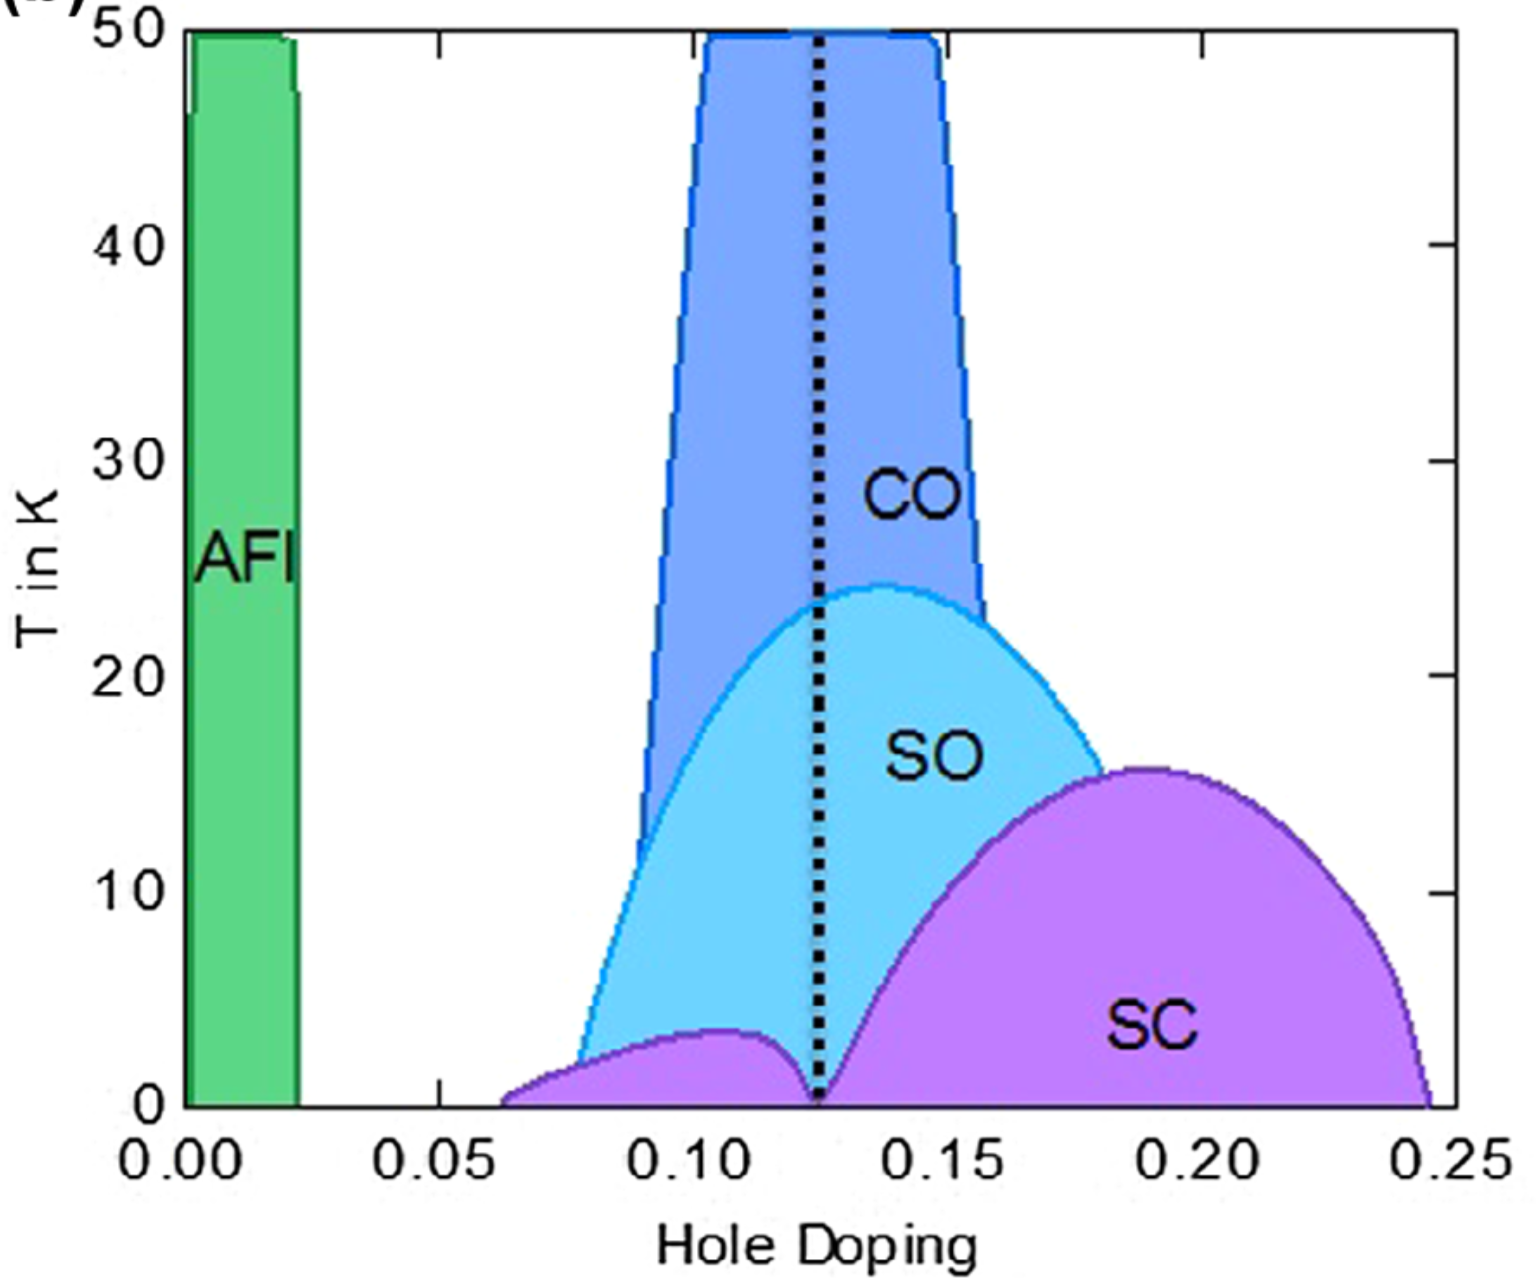
\includegraphics[width=0.5\hsize]{Introduction/phase_diagram2.eps}
  \end{center}
  \caption{銅酸化物超伝導体$\rm La_{1.8-x}Eu_{0.2}Sr_{x}CuO_4$の相図\cite{Cavalleri2018}}
  \label{fig:phase_diagram2}
\end{figure}

同様にMitranoらはフラーレンとアルカリ金属のインターカレーション$\rm K_3C_{60}$でも赤外光パルスにより過渡的な超伝導相が現れる可能性を示した\cite{Mitrano2016}。

これらはパルスを用いて秩序状態を破壊した結果に生じた超伝導であり、元素置換と異なった、非平衡過程を用いたアプローチである。この成果はパルス後の非平衡過程を用いて秩序状態の発現を阻害した点で、次に述べるパルス加熱・急冷を用いた手法と似ている。ただし赤外光パルスを用いたこの手法では過渡的な超伝導のみが実現されたが、次に述べるパルス加熱・急冷を用いた手法でが不揮発な超伝導が実現された。

\subsubsection{パルス加熱・急冷を用いた超伝導相の制御}
パルス加熱・急冷を用いて秩序状態を抑制し、準定常的な超伝導状態を実現した報告に関して述べる。

遷移金属ダイカルコゲナイドIrTe$_2$は銅酸化物超伝導体の母物質(Mott絶縁体)と同様にPbなどを元素置換すると超伝導を発現する\cite{IrTe2Pd_SC}。また低温で電荷が配列し電荷秩序状態となる点も、反強磁性秩序をもつ銅酸化物超伝導体の母物質と類似している。

大池らは電荷が配列し電荷秩序状態となった母物質のIrTe$_2$薄片を電流パルスにより加熱・急冷すると、急冷時に電荷秩序状態の発現が阻害され、競合する超伝導状態が現れることを示した\cite{oike}。図\ref{fig:phase_diagram2}にパルス加熱・急冷を用いた超伝導制御の概念図を示す。IrTe$_2$を通常の冷却率でゆっくり冷やす(徐冷)と電荷秩序状態となり、超伝導を示さない。しかしパルス後素早く冷やす(急冷)と電化秩序が現れずに超伝導となる。
\begin{figure}[!h]
    \begin{center}
   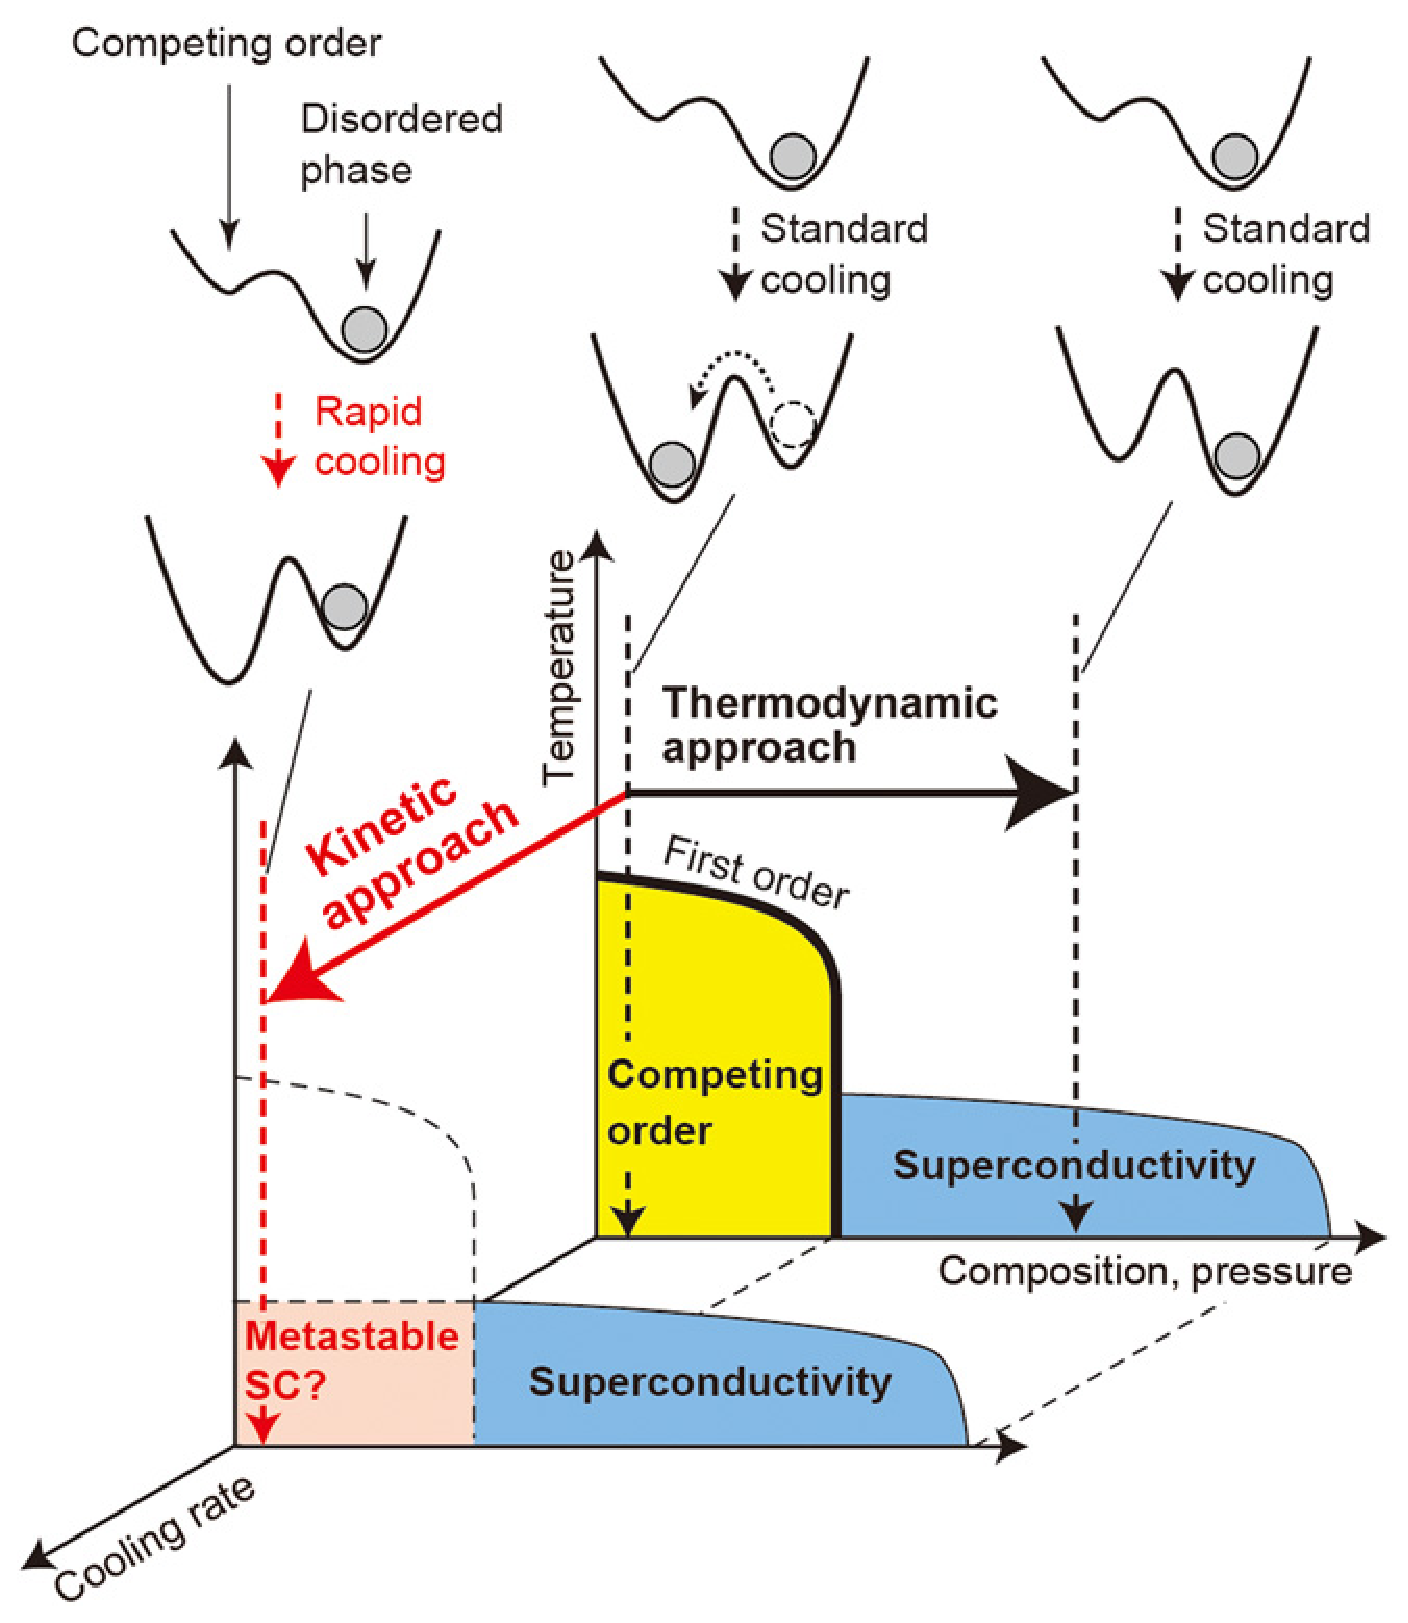
\includegraphics[width=0.6\hsize]{Introduction/kinetic_approach.eps}
  \end{center}
  \caption{非平衡過程を用いた相制御の概念図}
  \label{fig:kinetic_approach}
\end{figure}

急冷により超伝導が現れる条件は、冷却レートと試料の大きさによって決まる\cite{oike,Oike_size}。薄片試料を冷却レート$10^7$K/s以上で急冷したとき(図\ref{fig:kinetic_approach2}F,G)超伝導を示す。
\begin{figure}[!h]
    \begin{center}
   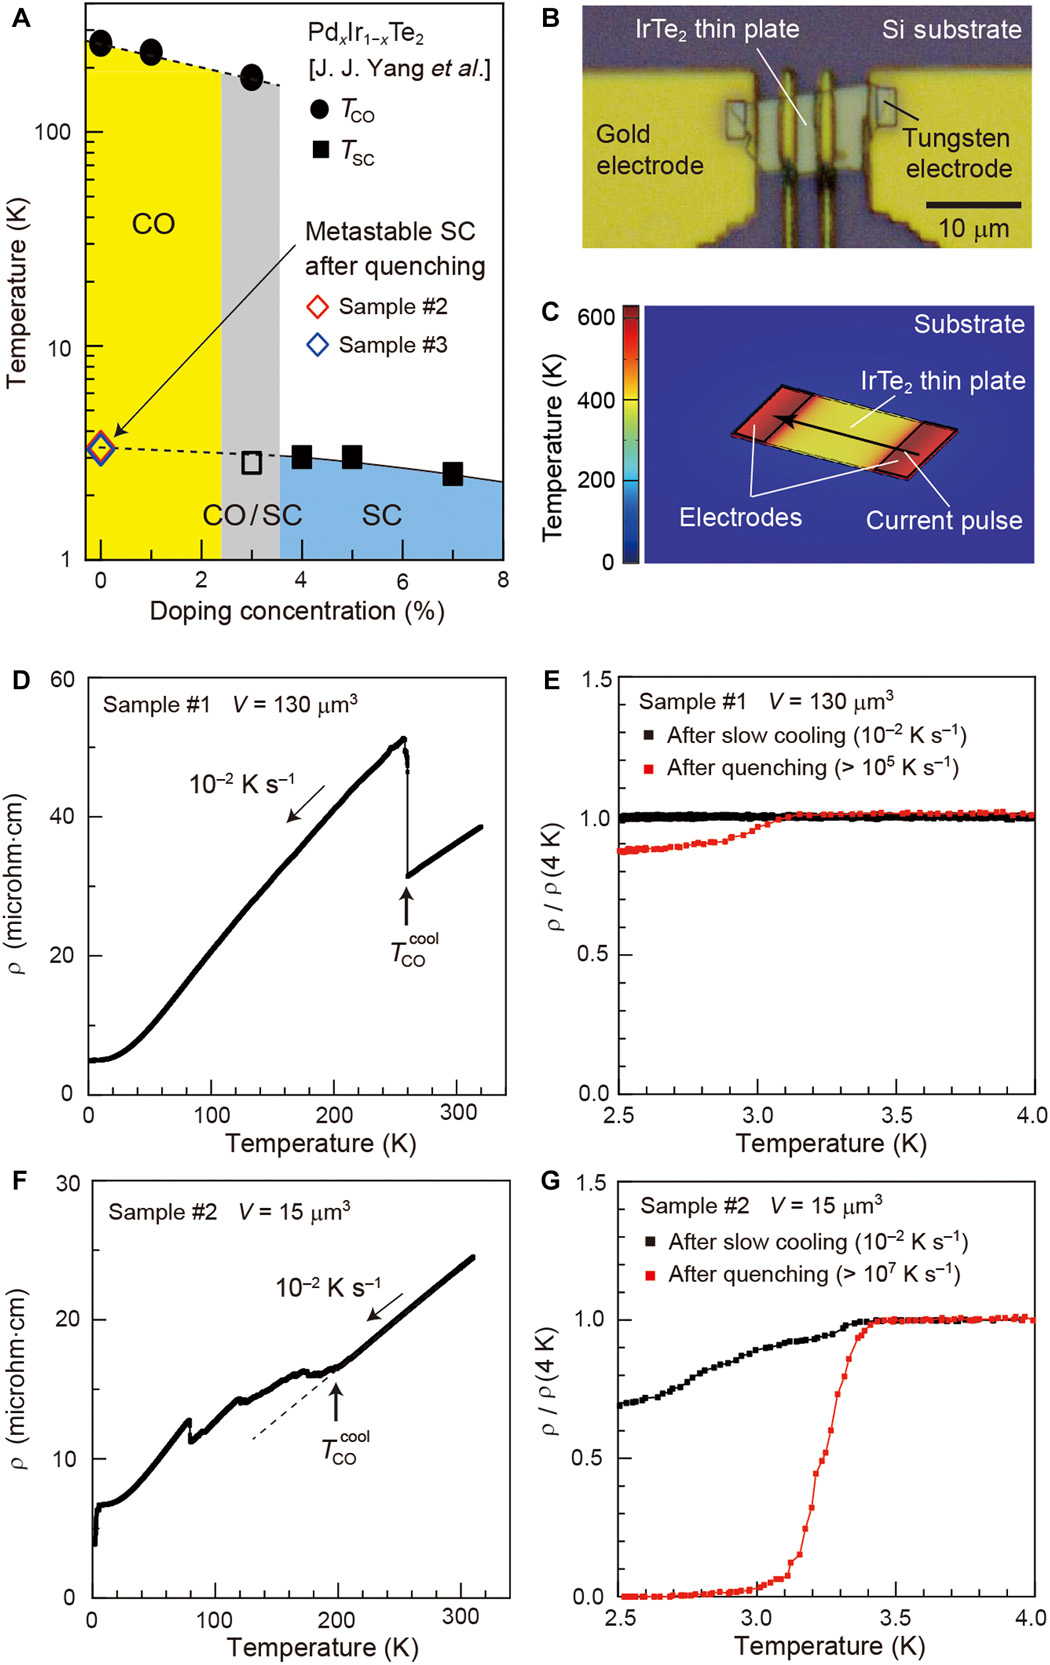
\includegraphics[width=0.6\hsize]{Introduction/kinetic_approach2.eps}
  \end{center}
  \caption{非平衡過程を用いた超伝導の発現}
  \label{fig:kinetic_approach2}
\end{figure}

この超伝導状態は準安定であり、数週間以上持続する。さらにパルス強度とパルス幅を適切に調整することで、超伝導から電荷秩序状態を復元できることも示した。これらは急加熱・急冷を用いて競合する秩序状態を抑制した結果に生じた超伝導であり、平衡過程からは到達できない状態(超伝導)を実現できる。

\subsection{スズ(Sn)のパルス加熱・急冷}
本実験では、IrTe$_2$で実現されたパルス加熱・急冷を用いた超伝導制御をスズに応用することを目指した。

スズは286.4Kより高温で正方晶の金属相(βスズ)が安定である。一方286.4Kより低温において立方晶の半導体相(αスズ)が安定だが、βスズを十分に早く冷却すると構造相転移できずβスズも準安定となる。このβスズは臨界温度3.7K以下で超伝導を示す。したがって冷却速度(温度履歴)をコントロールすれば、原理的に超伝導体と半導体間の制御・変換が可能である。

半導体スズと金属スズの特性は大きく異なる。半導体スズは低温で指数関数的に電気抵抗が大きくなるが、金属スズは臨界温度3.7K以下で超伝導を示し抵抗がゼロとなる。また光学的な性質も異なる。半導体スズはエネルギー0.018eV(4.4THz)以下の光を透過するが、金属スズは反射する。これらの性質から、半導体中の超伝導回路のパターニングは低損失な電気回路のみならず、プラズモニック回路や量子コンピュータなどに有用であることが期待できる。特にスズは地球上に豊富に存在する元素であり、融点が低く取り扱いやすく、また人体への毒性もない。応用の幅広さと取り扱いの簡単さから、パルス加熱・急冷による半導体スズと超伝導スズの変換は有用であることが期待できる。

\subsubsection{スズの基本的な物質特性}
スズは周期表において14族の元素である。図\ref{fig:group14}に14族の物質構造を示した。Geはスズのひとつ上の周期に属し、金属のPbはひとつ下の周期に属する。SiとGe、半導体のスズはダイアモンド構造をとる。金属のスズはPbと同様に金属的な高い導電性を示す。室温付近で金属と半導体のエネルギー差は小さく、どちらも安定に存在する。図\ref{fig:bandgaps}に14族半導体のバンドギャップ$\epsilon_g$と最近接原子間距離$R_{nn}$を示す\cite{Yonezawa}。最近接原子間距離$R_{nn}$が大きいほどバンドギャップは小さくなり、半導体スズはバンドが閉じるギリギリのところにあることが見て取れる。半導体スズのバンドギャップは0.08eVと非常に小さい。
\begin{figure}[!h]
 \begin{minipage}{0.4\hsize}
  \begin{center}
   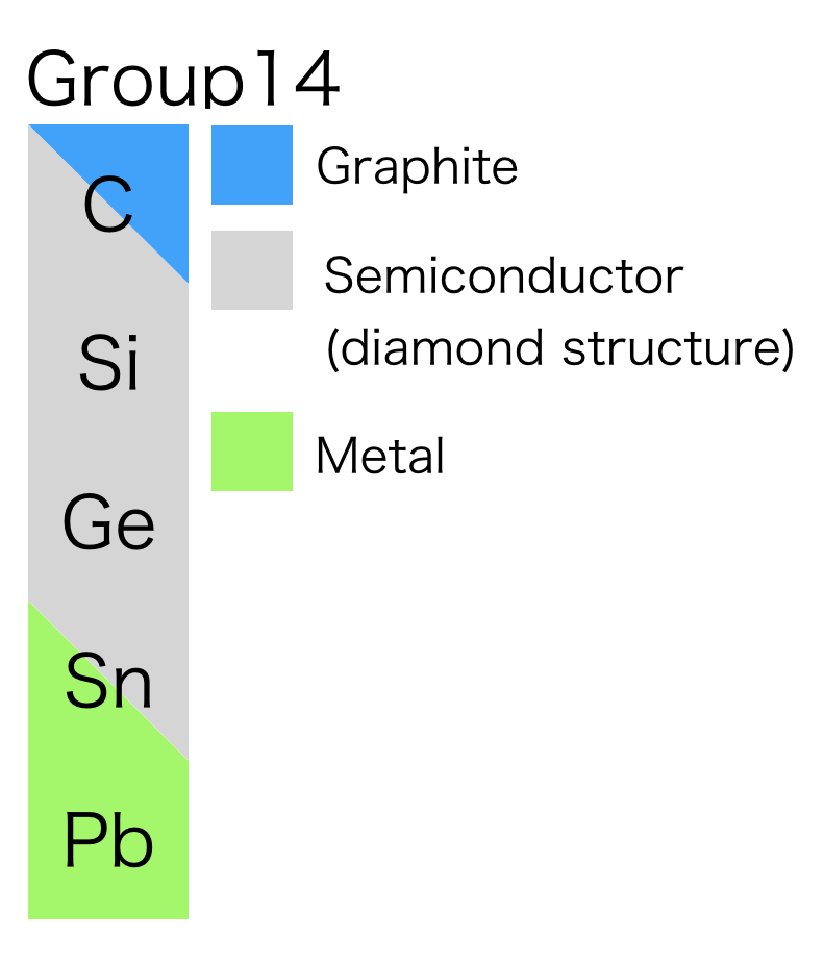
\includegraphics[width=\hsize]{Introduction/group14.eps}
  \end{center}
  \caption{14族元素の相}
  \label{fig:group14}
 \end{minipage}
 \begin{minipage}{0.6\hsize}
  \begin{center}
   
\includegraphics[width=\hsize]{Introduction/bandgaps.eps}
  \end{center}
  \caption{14族半導体のバンドギャップ$\epsilon_g$と最近接原子間距離$R_{nn}$\cite{Yonezawa}}
  \label{fig:bandgaps}
 \end{minipage}
\end{figure}


\subsubsection{半導体-金属転移}
温度を上げると半導体スズの$R_{nn}$はさらに大きくなり、バンドが閉じ金属的になる。この半導体-金属転移はブロッホ・ウィルソン転移(タイプ2)と呼ばれる\cite{Yonezawa}。

αスズとβスズの構造転移には27\%程度の大きな体積変化が伴う。したがって、核生成は試料の内部より表面から始まりやすい\cite{Cornelius}。

図\ref{fig:alpha-to-beta}と図\ref{fig:beta-to-alpha}にそれぞれ、αスズからβスズへの転移にかかる時間と、βスズからαスズへの転移にかかる時間を示す\cite{Nogita}。
図\ref{fig:alpha-to-beta}から、αスズからβスズへの転移は温度が転移温度よりも十分に高ければ3分未満で進行する。一方、図\ref{fig:beta-to-alpha}から、
最速でもβスズからαスズへの転移は、それ以上の時間がかかる可能性が示唆される。
αスズとβスズは室温で安定である。
\begin{figure}[!h]
 \begin{minipage}{0.5\hsize}
  \begin{center}
   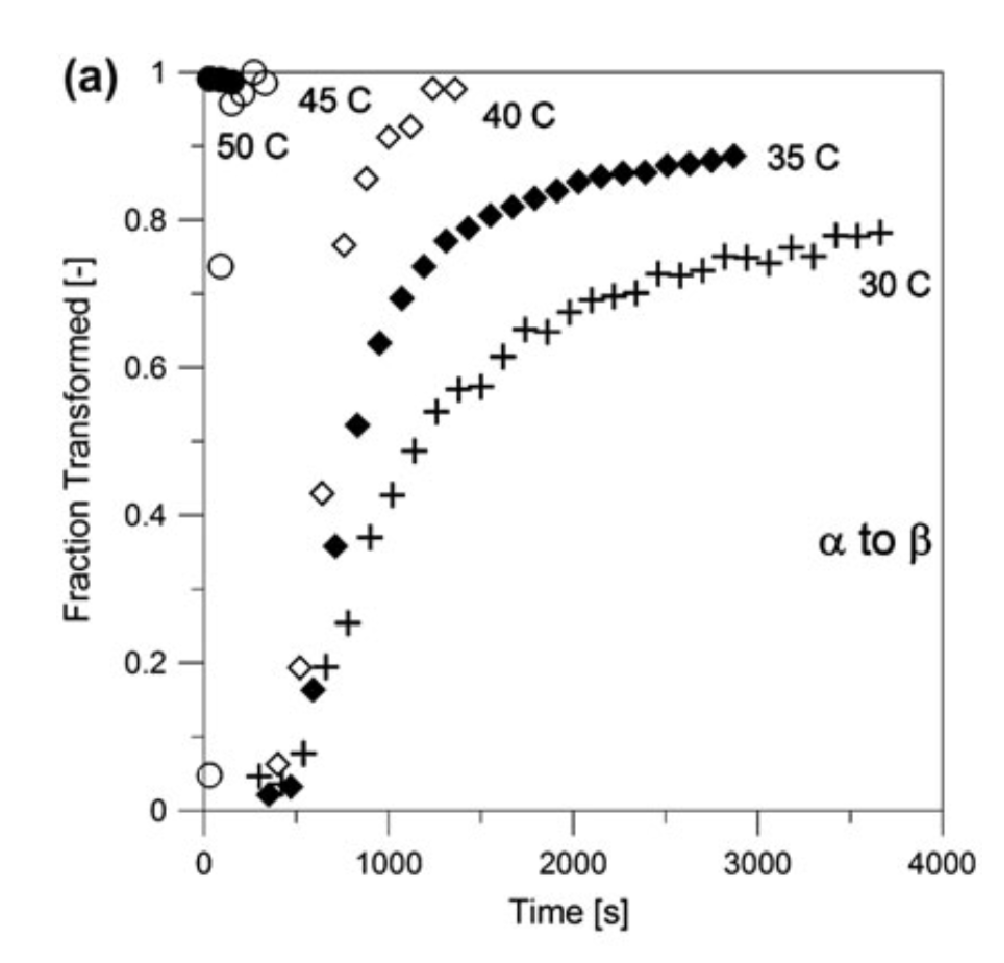
\includegraphics[width=\hsize]{Introduction/alpha-to-beta.eps}
  \end{center}
  \caption{αスズからβスズへの転移にかかる時間}
  \label{fig:alpha-to-beta}
 \end{minipage}
 \begin{minipage}{0.5\hsize}
    \begin{center}
   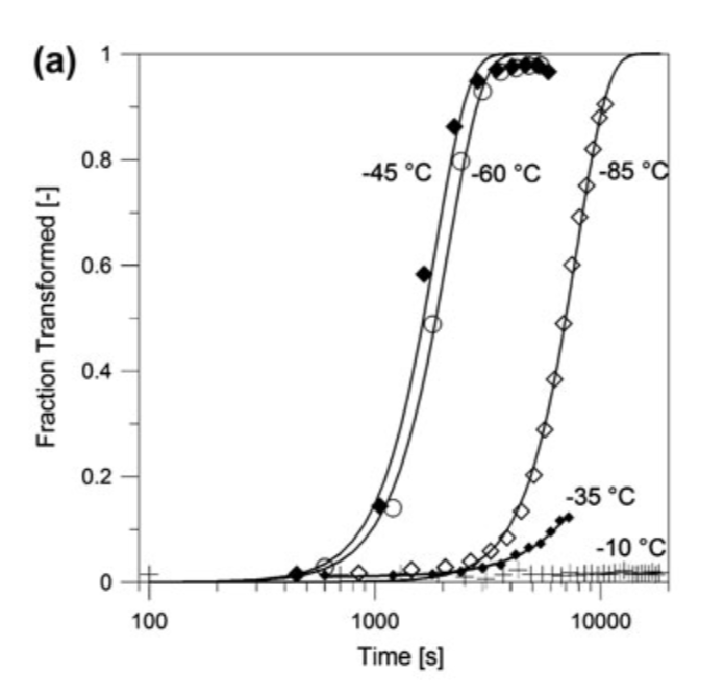
\includegraphics[width=\hsize]{Introduction/beta-to-alpha.eps}
  \end{center}
  \caption{βスズからαスズへの転移にかかる時間}
  \label{fig:beta-to-alpha}
 \end{minipage}
\end{figure}

\begin{figure}[!h]
    \begin{center}
   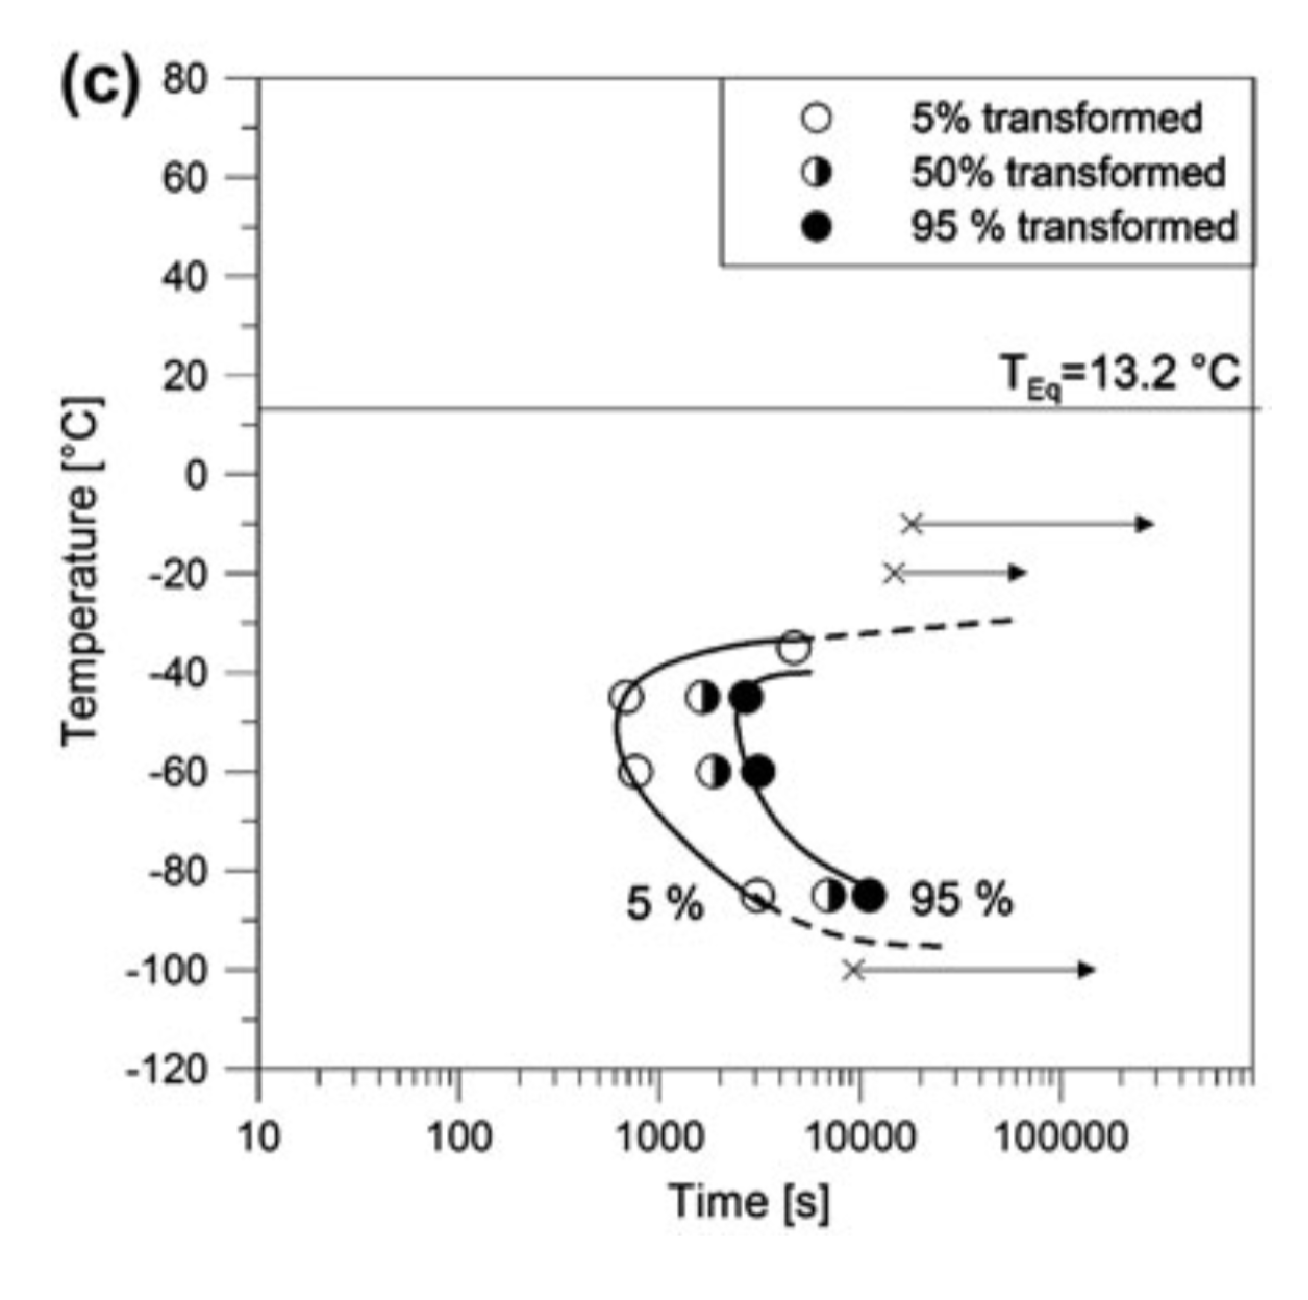
\includegraphics[width=0.6\hsize]{Introduction/TTT.eps}
  \end{center}
  \caption{温度と$\beta-\alpha$転移時間の関係(TTT)\cite{Nogita}}
  \label{fig:TTT}
\end{figure}

αスズは半導体(バンドギャップエネルギー$\rm E_G=0.018eV$)であり低温になればなるほど抵抗が大きい。一方、βスズは金属であり低温になればなるほど抵抗が小さくなる。また室温付近でαスズとβスズの抵抗を比較してもβスズの方が2桁程度小さい。したがって、抵抗測定を行うと相転移が起こったかどうかもわかる。
\begin{figure}[!h]
    \begin{center}
   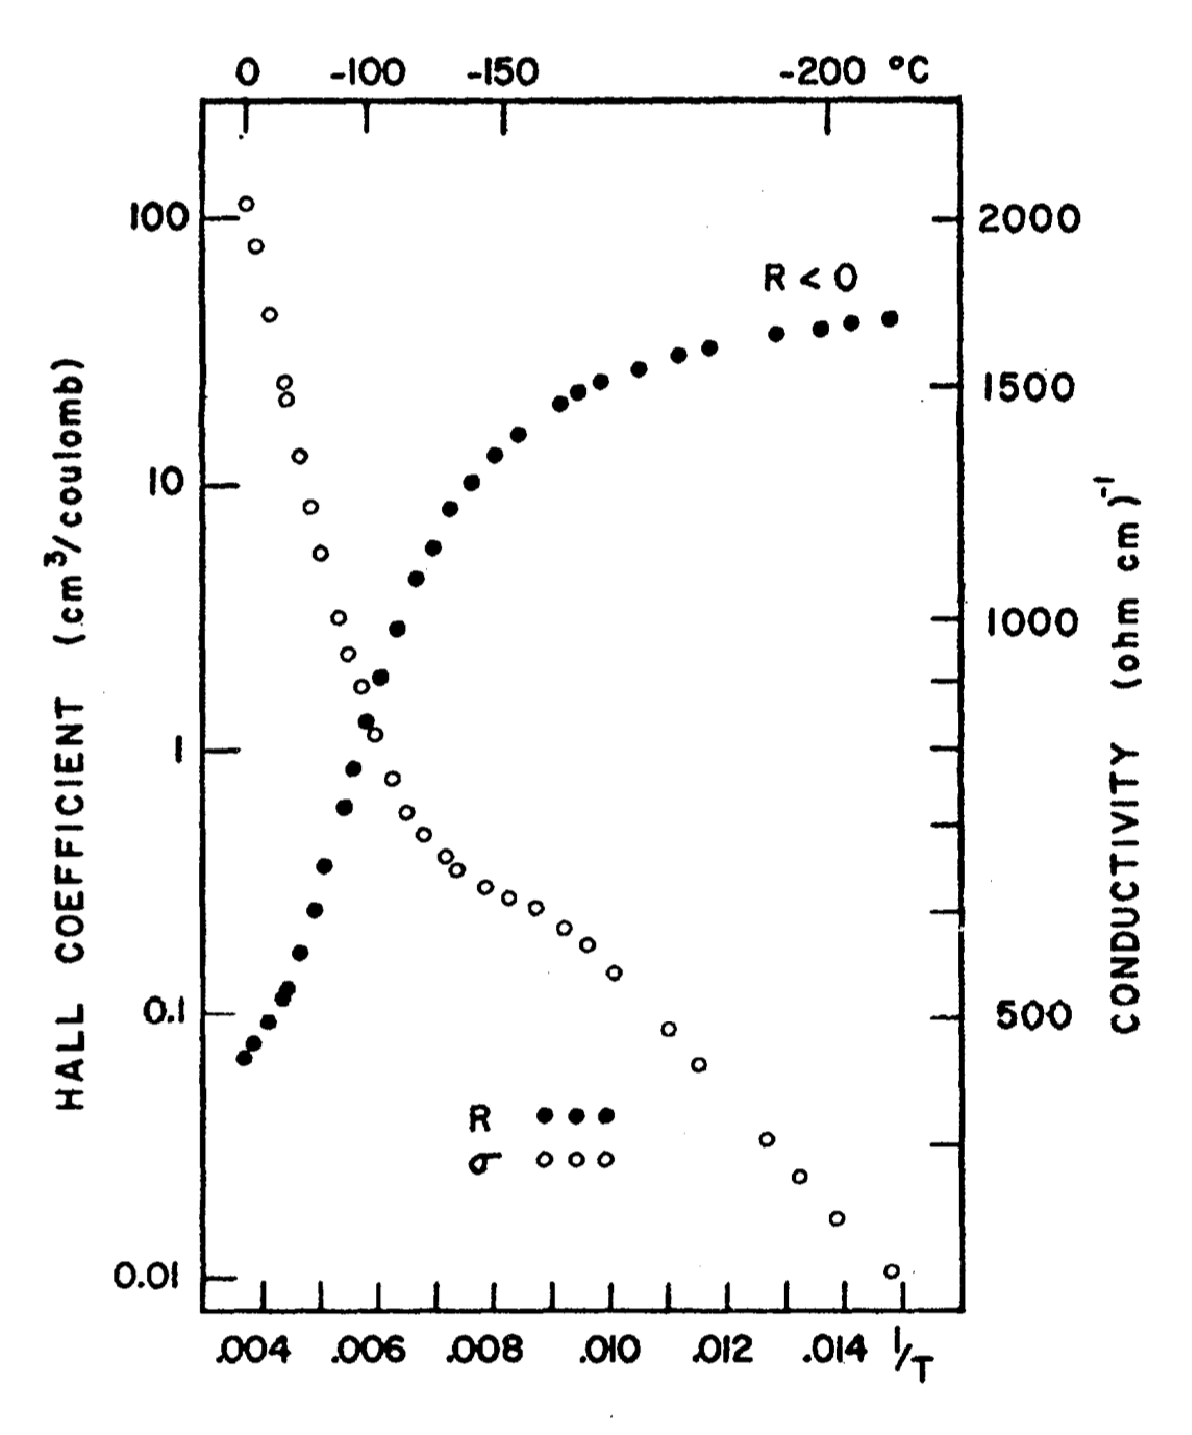
\includegraphics[width=0.6\hsize]{Introduction/conductivity.eps}
  \end{center}
  \caption{温度とホール係数、導電率の関係\cite{Kohnke}}
  \label{fig:conductivity}
\end{figure}

%αスズは室温と200K以下で安定

%金属と半導体の抵抗の温度依存性(グラフ)

%半導体抵抗のアノマリ

βスズは金属光沢があり、可視域を吸収するαスズに比べ反射率が大きい。図\ref{fig:Sn-Alpha-Beta}にαスズとβスズの外観を示す\cite{wiki}。見た目が異なることから空間的なα相とβ相を測定することができる。
さらにαスズは立方晶であり、βスズは正方晶である。これらの対称性の違いから、付録\ref{sec:reflectance}に示すように偏光顕微鏡から転移が観察できる\cite{Matvienko}。
\begin{figure}[!h]
    \begin{center}
   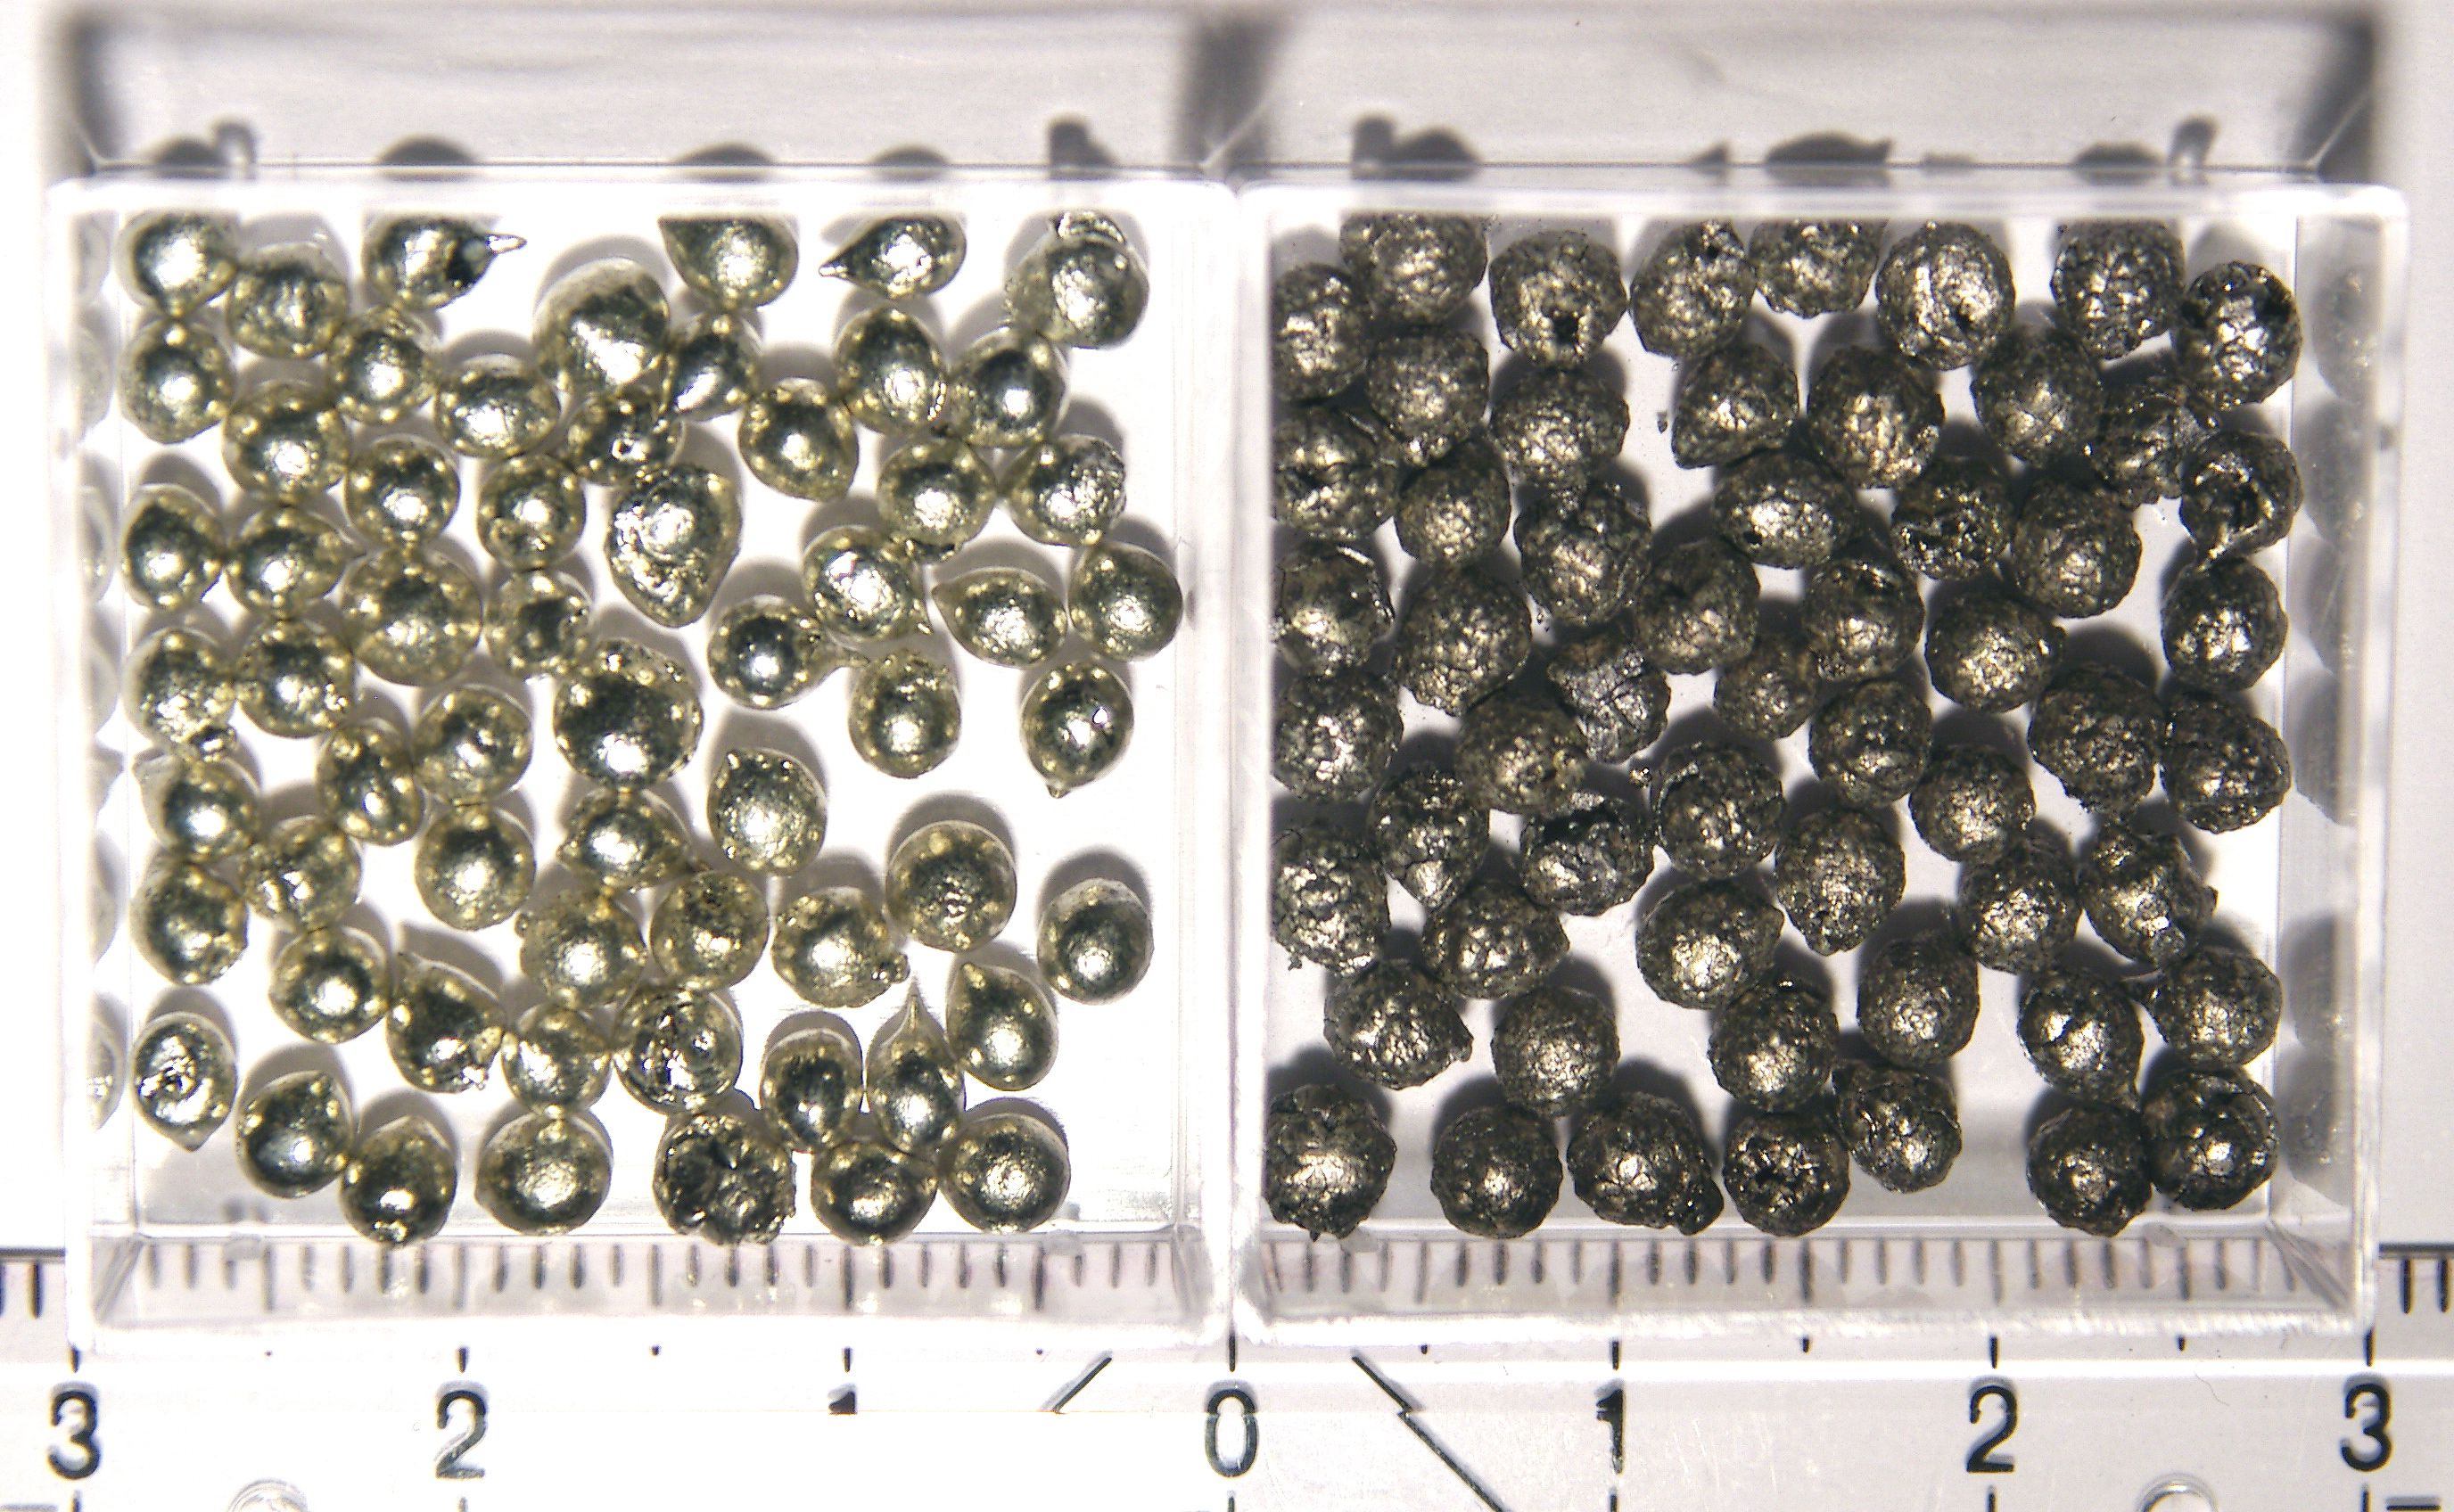
\includegraphics[width=0.5\hsize]{Introduction/Sn-Alpha-Beta.eps}
  \end{center}
  \caption{αスズとβスズの外観 (左: βスズ; 右: αスズ)}
  \label{fig:Sn-Alpha-Beta}
\end{figure}

\subsection{Sn-Ge合金試料の特性}
図\ref{fig:GeSn_phase}にGe-Snコンポジット(合金)の相図を示す\cite{Olesinski1984}。共晶型の相図であり、スズ-Ge共晶点に置けるGe固溶の限界は0.3\%程度と言われている\cite{Thurmond1960}。
\begin{figure}[!h]
 \begin{minipage}{\hsize}
    \begin{center}
   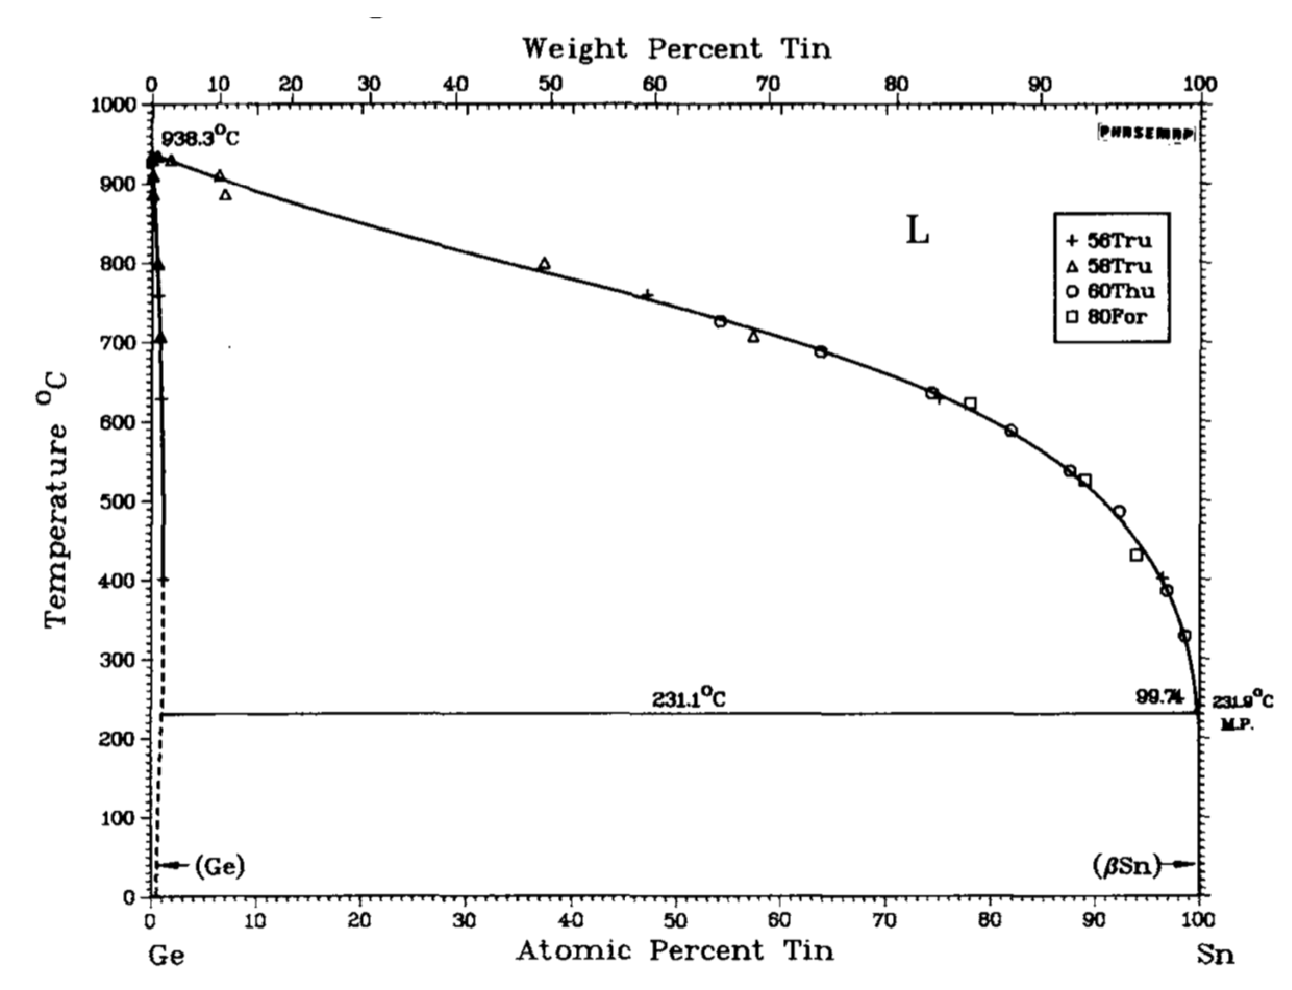
\includegraphics[width=0.7\hsize]{Introduction/GeSn_phase.eps}
  \end{center}
  \caption{Ge-Sn合金の相図\cite{Olesinski1984}}
  \label{fig:GeSn_phase}
 \end{minipage}
 \begin{minipage}{\hsize}
    \begin{center}
   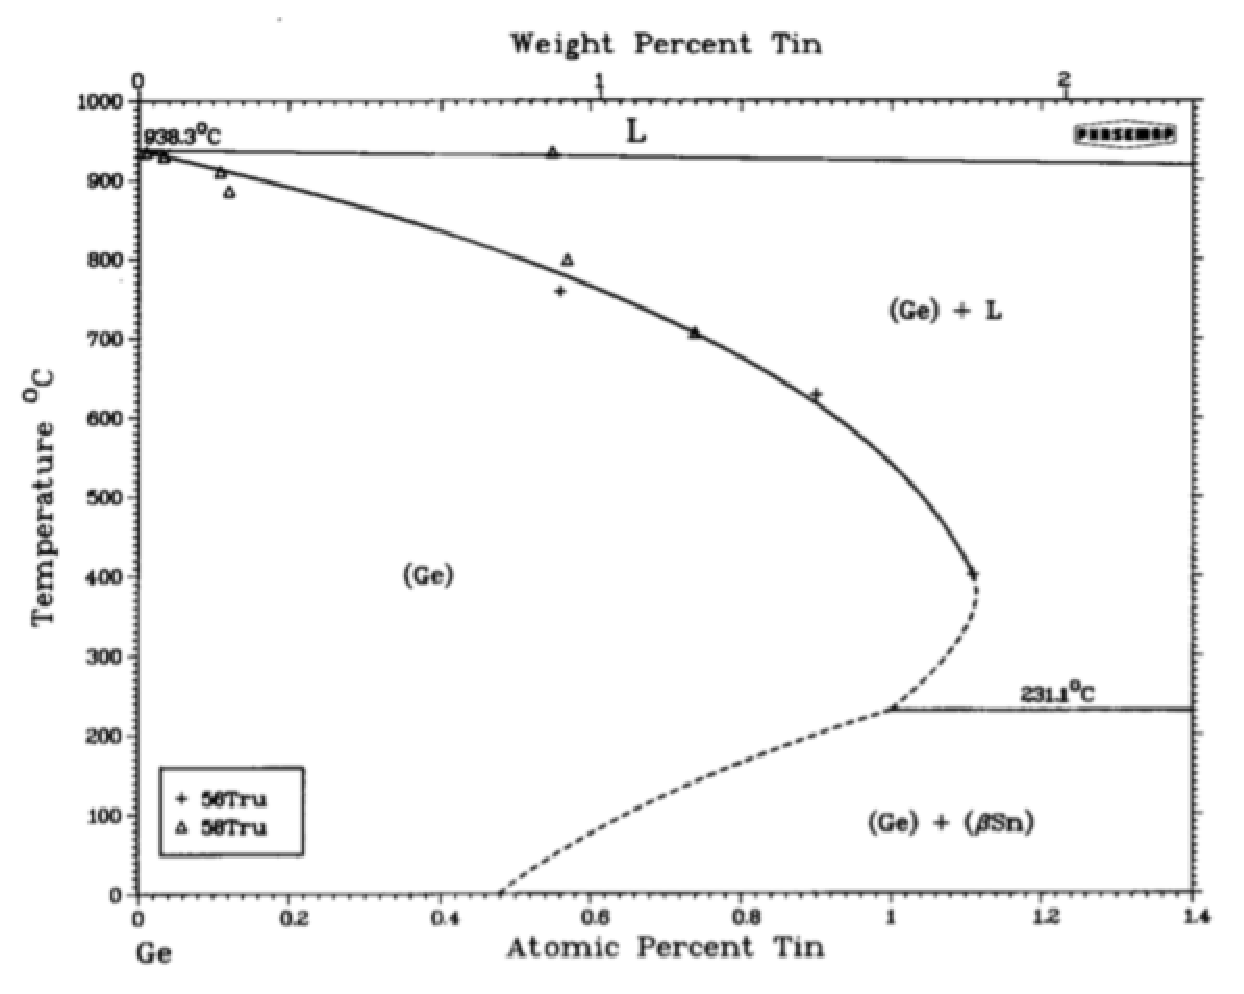
\includegraphics[width=0.7\hsize]{Introduction/GeSn_phase2.eps}
  \end{center}
  \caption{Ge-Sn合金の相図(Geリッチ領域を拡大したもの)\cite{Olesinski1984}}
  \label{fig:GeSn_phase2}
   \end{minipage}
\end{figure}

SiとGeと半導体スズはすべて同一のダイアモンド構造をとることから、半導体スズにSiやGeを少量添加すると安定化することが示唆されている\cite{Ewald1954,Gallerneault1983}。

図\ref{fig:Ge_Stabilized_Sn}にGe添加量と半導体-金属転移温度の関係を示した\cite{Vnuk1984}。Ge添加量を1\%程度まで増やすと転移温度が大きくなることが見て取れる。

一方、Matvienkoらの研究\cite{Matvienko}によると、β相からα相への変換はα-β相界面でのβ相の塑性変形が重要な役割を果たしており、Geを添加するとβ相中の欠陥の拡散が遅くなりα-β変換が阻害される。その結果、図\ref{fig:Ge_content}に示したように、Ge添加量とα-β相界面の移動速度の関係を示した\cite{Matvienko}。Ge添加量が0 at. \%から0.3 at. \%(2 wt. \%)程度までは、添加量を多くすると転移速度が遅くなってゆくことが見て取れる。
%0.3mol\%= 0.003*32/(0.997*50+0.003*32)質量\%
\begin{figure}[!h]
 \begin{minipage}{0.4\hsize}
    \begin{center}
   \includegraphics[width=\hsize]{Introduction/Ge_Stabilized_Sn.eps}
  \end{center}
  \caption{Ge添加量とスズの$\alpha-\beta$転移温度\cite{Vnuk1984}}
  \label{fig:Ge_Stabilized_Sn}
 \end{minipage}
 \begin{minipage}{0.6\hsize}
    \begin{center}
   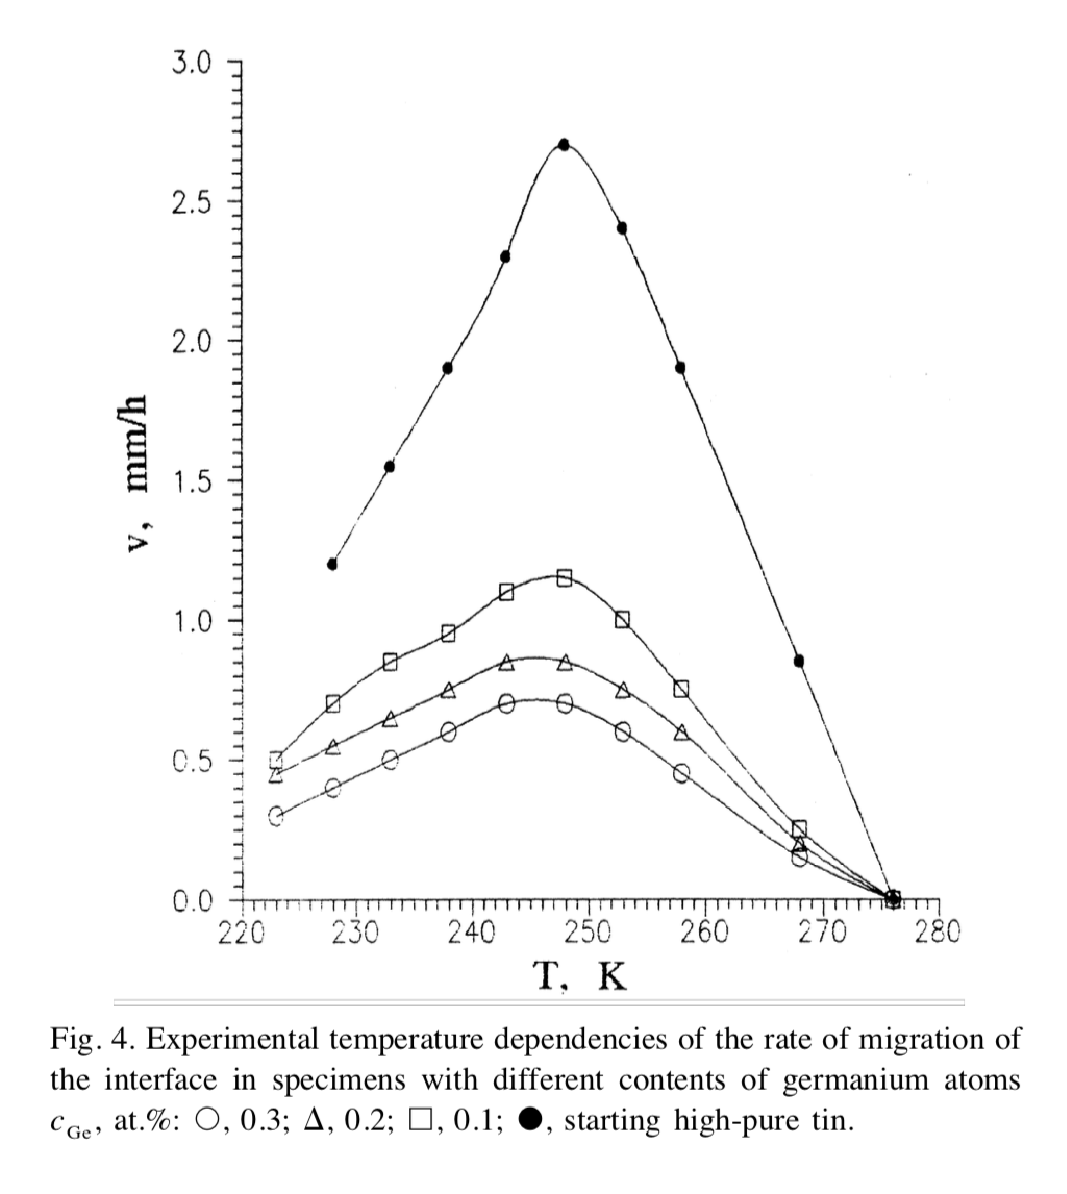
\includegraphics[width=\hsize]{Introduction/Ge_content.eps}
  \end{center}
  \caption{Ge添加量と$\beta-\alpha$転移速度の関係\cite{Matvienko}}
  \label{fig:Ge_content}
   \end{minipage}
\end{figure}
\clearpage

\subsection{研究の目的}
1-2節で述べたように、IrTe$_2$に対してパルス加熱・急冷を適用すると、準安定状態として超伝導状態を生成できることが知られている。しかし、この原理はIrTe$_2$のみで実証されたものであり、様々な物質系における超伝導生成に適用できる原理であるかは、非自明な問題である。また、IrTe$_2$における超伝導状態の生成は、常伝導金属を超伝導に変換するものであり、抵抗の絶対値の変化は小さい。

そこで本研究では、パルス加熱・急冷を用いた超伝導生成法を、スズに適用することを考えた。1-3節で述べたように、スズの最安定状態は、286.4K以上では金属スズ(βスズ) 、286.4K以下では半導体スズ(αスズ)であることが知られている。また、金属スズを十分に早く冷却すると半導体スズへの構造相転移を動的に避けることができ、3.7K 以下では金属スズが超伝導転移を示す。したがって、半導体スズに対してパルス加熱・急冷を適用すると、IrTe$_2$の研究において実証された原理に基づいて、超伝導スズに変換できることが期待される。これにより、パルス加熱・急冷を用いた生成法が複数の物質系に適用できることを実証し、大きな抵抗変化を伴う超伝導生成を実現することを、本研究の目的とした。
\clearpage
